\documentclass[landscape]{article}

\pagenumbering{gobble}
\usepackage{tikz}
\usetikzlibrary{calc,shapes,positioning}
\usetikzlibrary{arrows}
\newcommand{\midarrow}{\tikz \draw[-triangle 90] (0,0) -- +(.1,0);}
\usepackage{bm}
\newcommand{\Ss}{\mathcal{S}}
\newcommand{\Tt}{\mathcal{T}}

\usepackage{amsmath,graphicx}
\newcommand{\ubar}[1]{\mkern2mu\underline{\mkern-2mu #1\mkern-2mu}\mkern2mu}
\newcommand{\ubm}[1]{\ubar{\bm{#1}}}
% \newcommand{\ubmr}[2]{\ubar{\bm{#1}}^{#2}}

\begin{document}

\begin{figure}

  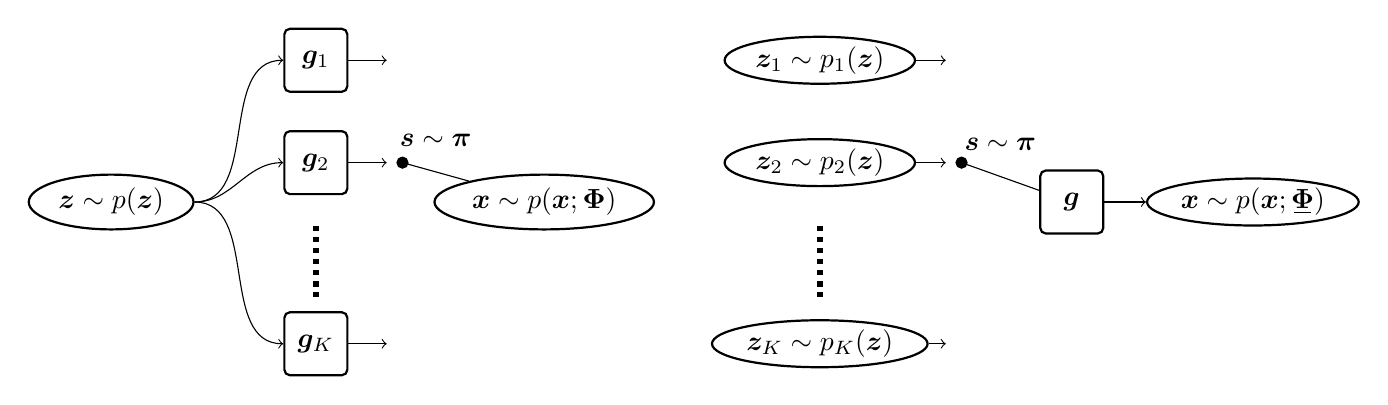
\begin{tikzpicture}


    \begin{scope}[xshift=-2cm]
      \tikzstyle{enode} = [thick, draw=black, ellipse, inner sep = 2pt,  align=center]
      \tikzstyle{nnode} = [thick, rectangle, rounded corners = 2pt,minimum size = 0.8cm,draw,inner sep = 2pt]
      \node[enode] (z) at (0,0) {$\bm{z}\sim p(\bm{z})$};
      \node[enode] (x) at (5.5,0){$\bm{x}\sim p(\bm{x}; \bm{\Phi})$};
      % \node at (5.2,-1) {$p(\bm{x};\bm{\Phi}) = \textstyle\sum_{k=1}^K \pi_k  p_k(\bm{x})$};
      \node[nnode] (g1) at (2.6,1.8) {$\bm{g}_1$};
      \node[nnode] (g2) at (2.6,0.5) {$\bm{g}_2$};
      \node[nnode] (gk) at (2.6,-1.8) {$\bm{g}_K$};
      \draw[dotted,line width=2pt] (2.6,-0.3) -- (2.6,-1.2);
      \draw[->] (z) [in= 180, out =0] to (g1);
      \draw[->] (z) [in= 180, out =0] to (g2);
      \draw[->] (z) [in= 180, out =0] to (gk);
      \filldraw[->] (3.7, 0.5)circle (2pt) -- node[above=0.2]{$\bm{s}\sim \bm{\pi}$} (x) ;
      % \draw[->] (3,-0.8) -- (3.5, -0.8);
      \draw[->] (g1) -- (3.5,1.8);
      \draw[->] (g2) -- (3.5, 0.5);
      \draw[->] (gk) -- (3.5, -1.8);
    \end{scope}


    \begin{scope}[xshift=7cm, yshift=0cm]
      \tikzstyle{enode} = [thick, draw=black, ellipse, inner sep = 1pt,  align=center]
      % \tikzstyle{nnode} = [thick, rectangle, rounded corners = 1pt,minimum size = 1.2cm,draw,inner sep = 2pt]
      \tikzstyle{nnode} = [thick, rectangle, rounded corners = 2pt,minimum size = 0.8cm,draw,inner sep = 2pt]
      \node[enode] (z1) at (0,1.8) {$\bm{z}_1\sim p_1(\bm{z})$};
      \node[enode] (z2) at (0,0.5){$\bm{z}_2\sim p_{2}(\bm{z})$};
      \node[enode] (zK) at (0,-1.8) {$\bm{z}_K\sim p_{K}(\bm{z})$};
      \node[enode] (x) at (5.5,0){$\bm{x}\sim p(\bm{x};\ubar{\bm{\Phi}})$};
      % \node at (3,-1){$p(\bm{z}) = \sum_k\pi_kp_k(\bm{z})$};
      \node[nnode] (g) at (3.2,0) {$\bm{g}$};
      \draw[dotted,line width=2pt] (0,-0.3) -- (0,-1.2);
      \filldraw[->] (1.8, 0.5)circle (2pt) -- node[above=0.2]{$\bm{s}\sim \bm{\pi}$} (g) ;
      \draw[->] (z1) -- (1.6, 1.8);
      \draw[->] (z2) -- (1.6, 0.5);
      % \draw[->] (1,-0.5) -- (1.8, -0.5);
      \draw[->] (zK) -- (1.6, -1.8);
      % \draw[->] (z1) [in=180,out=0]  to node[right]{$\pi_1$} (g);
      % \draw[->] (z2) [in=180,out=0]  to node[above]{$\pi_2$} (g);
      % \draw[->,dashed] (zK) [in=180,out=0]  to node[right]{$\pi_K$} (g);
      \draw[->] (g) to (x);
    \end{scope}

  \end{tikzpicture}


\end{figure}


\end{document}
%%% Local Variables:
%%% mode: latex
%%% TeX-master: t
%%% End:
